\section{Experiment}

\begin{figure*}
    \centering
    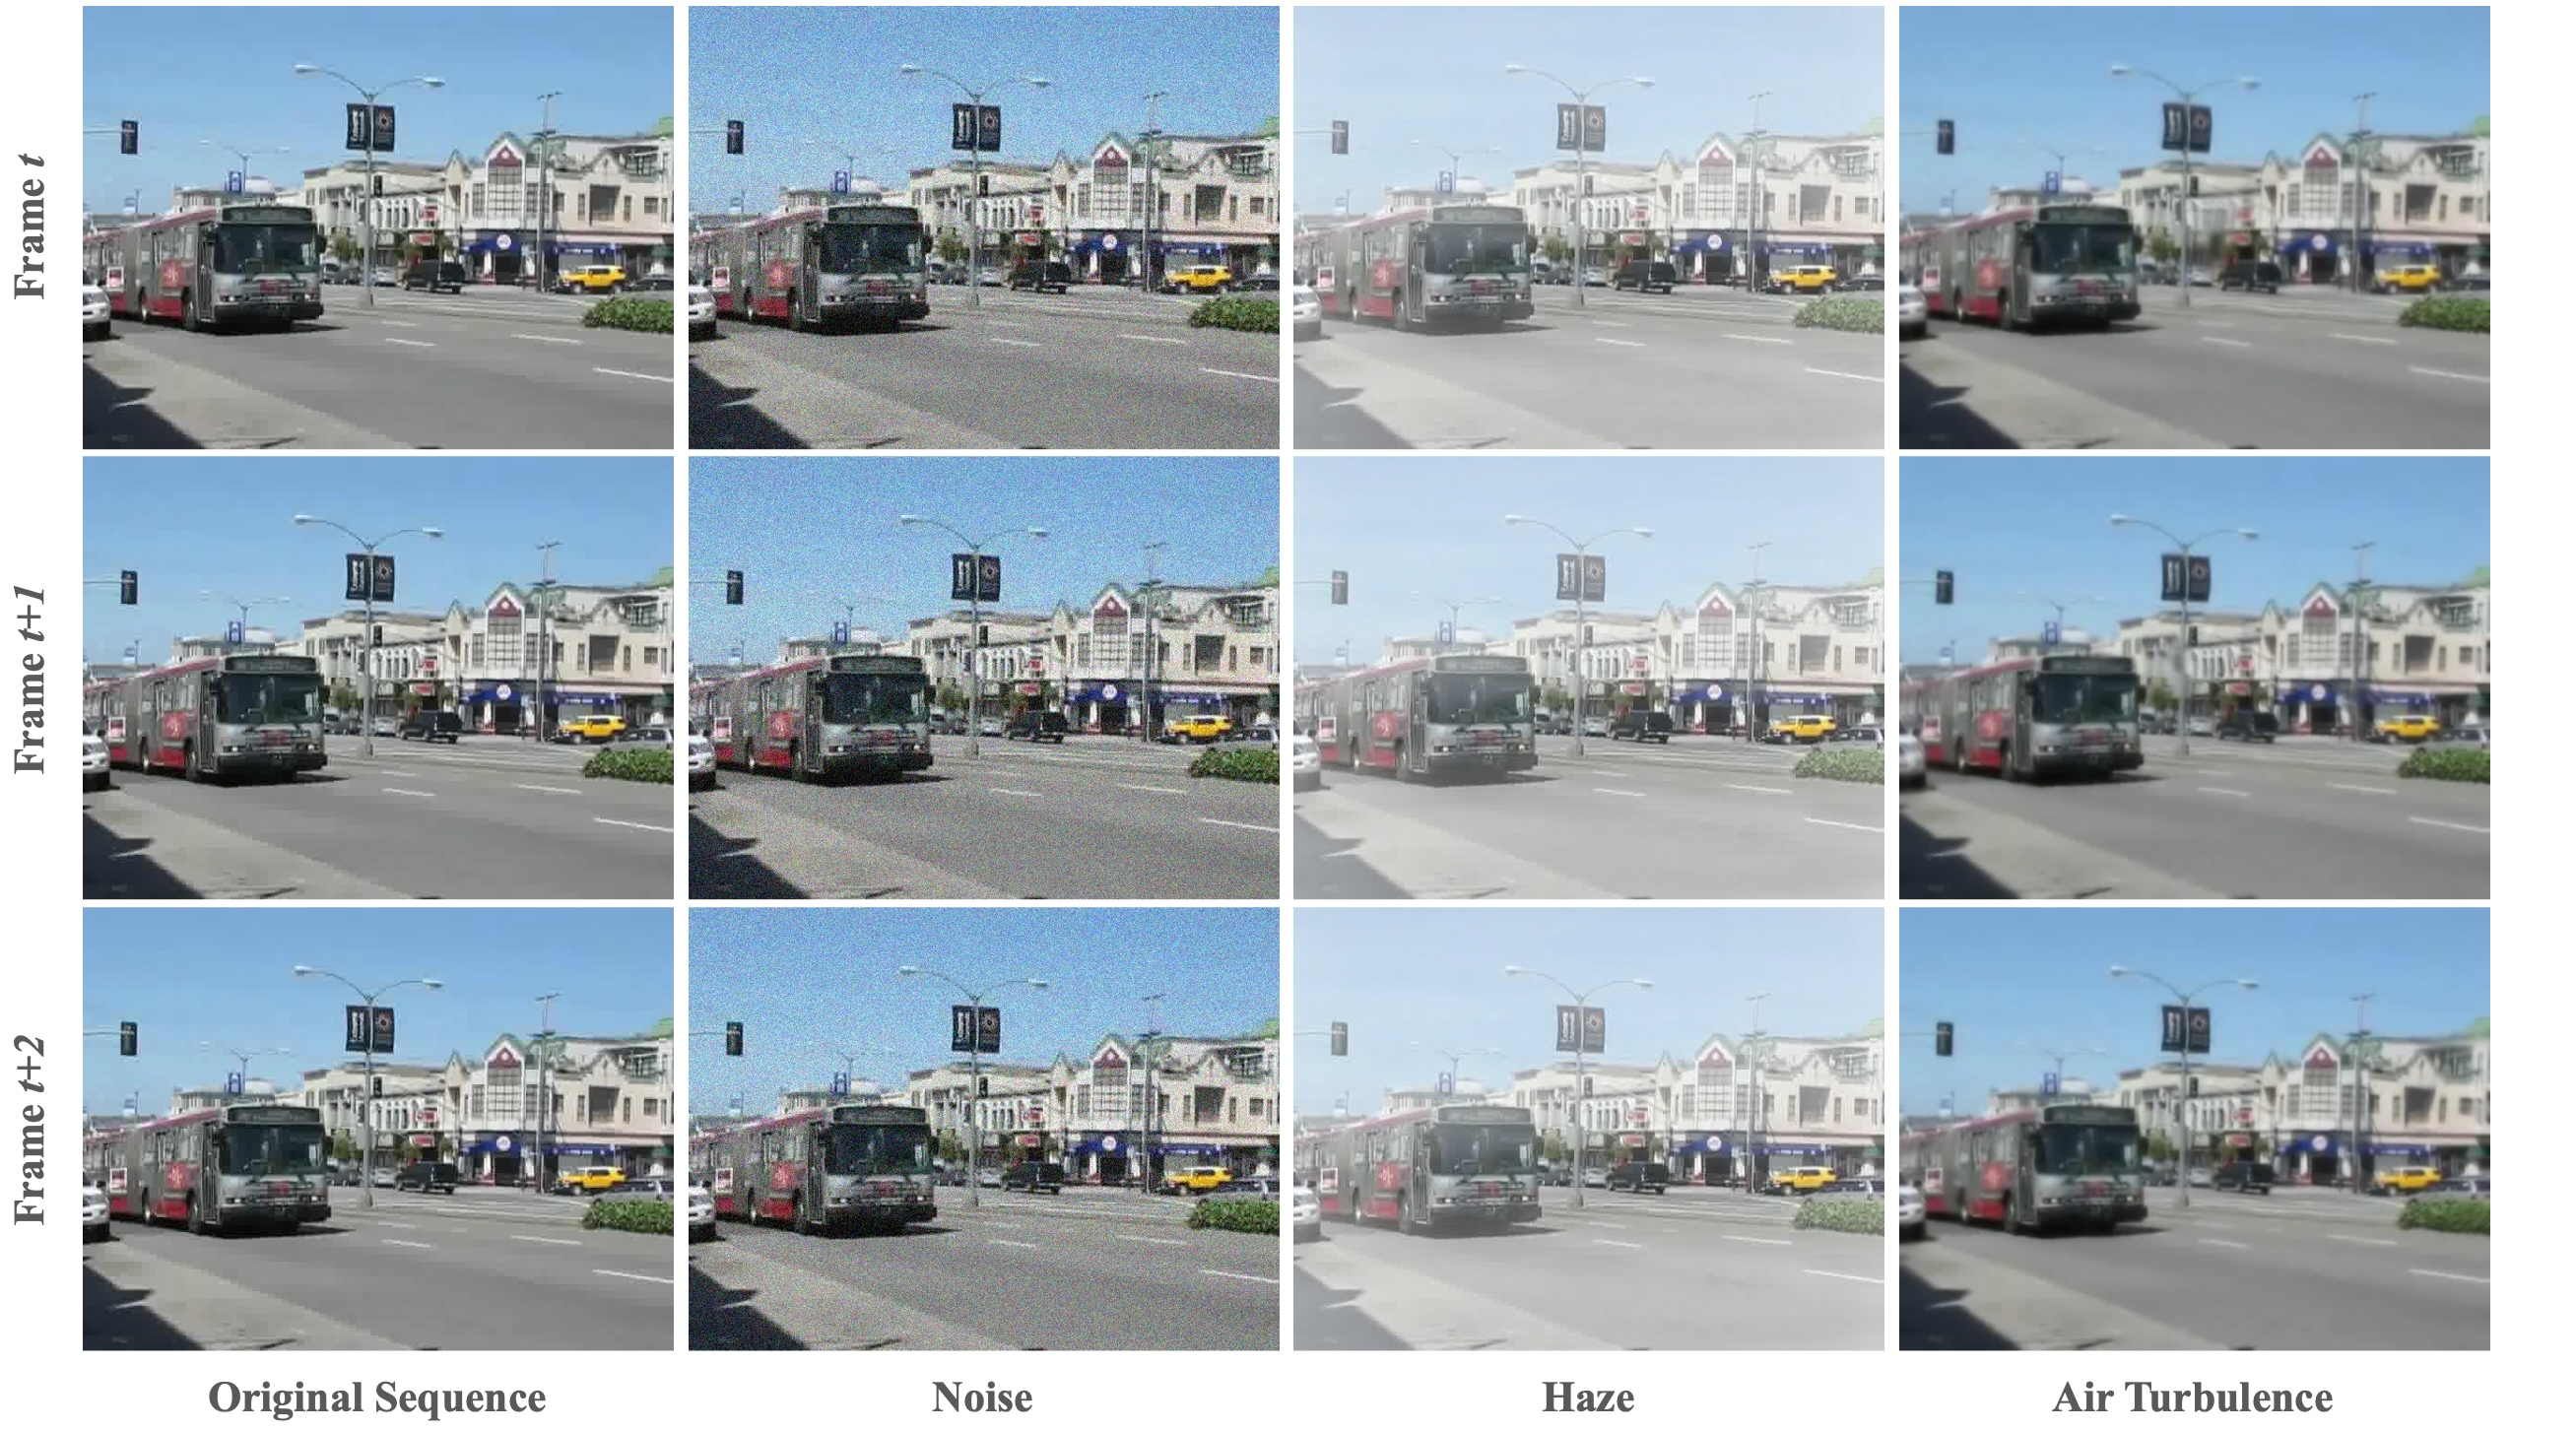
\includegraphics[width = 0.99\linewidth]{figures/test_sample.jpg}
    \caption{A snippet of the ImageNetVOD dataset and three forms of degradation. The original frames are from the testing video \textit{ILSVRC2015\_test\_00028000.mp4} and $t=32$.}
    \label{fig:test_sample}
\end{figure*}

\subsection{Adverse image condition synthesis}
\label{synthesis}
Real-world VOD often faces the challenge of domain gaps caused by adverse image conditions. Because of the complexity of image degradation, testing domain adaptation algorithms under various conditions is desired. However, appropriate datasets for testing the domain adaptation algorithm for VOD models trained on the ImageNetVOD dataset are unavailable. In this work, we synthesized videos in three common imaging conditions: noise, air turbulence, and haze. Each video has its distinct degradation parameter, with the profile varies temporally. A sample image sequence from the original dataset and the associated three degraded sequences are shown in Fig. \ref{fig:test_sample}. The unsupervised property of the algorithm guarantees that our method will be effective in real-world unknown degradations. The simulation of the three adverse image conditions is described below:

\noindent \textbf{Noise.} Noise is the predominant degradation in the low-light conditions. The noise in our experiment is modeled with:
\begin{equation}
    \widetilde{I}(h,w,t) = I(h,w,t) + n(h,w,t),
\end{equation}
\noindent where $I$ is the input image sequence, $\widetilde{I}$ is the degraded image sequence, $h$, $w$, and $t$ are the sequence's height, width, and frame indices. $n(h,w,t)\sim \mathcal{N}(0, \sigma^2)$ is the Gaussian noise. We randomly sample the variance of the noise in $\sigma^2\in [10/255, 50/255]$. Each sequence has its distinct variance.

\noindent \textbf{Air Turbulence.} In long-range imaging conditions, air turbulence may affect the performance of computer vision models significantly \cite{Liu_2024_WACV}. The air turbulence primarily causes random pixel displacement and spatially varying blur on the image \cite{chan2023computational}. We utilized the popular P2S simulator \cite{chimitt2020simulating, Mao_2021_ICCV} to synthesize the degraded video:
\begin{equation}
    \widetilde{I}(h,w,t) = \text{P2S}(I(h,w,t); n(h,w,t)).
\end{equation}
The P2S simulator converts the Gaussian random seed $n$ to spatially varying pixel displacement and blur. Inspired by \cite{chimitt2022real, zhang2022imaging}, we applied the temporal correlation and varying kernel size to improve the diversity and fidelity of the synthetic turbulence. Each image sequence has a distinct turbulence strength and profile.

\noindent \textbf{Haze.} Haze is a crucial adverse image condition in VOD application scenarios, especially in surveillance systems and automated driving. The hazy video can be modeled with the transmission function \cite{cai2016dehazenet}:
\begin{equation}
    \widetilde{I}(h,w,t) = I(h,w,t)e^{-\beta d(h,w,t)} + A(1-e^{-\beta d(h,w,t)} ),
\end{equation}
\noindent where $e^{-\beta d(h,w,t)}$ is the transmission rate, $\beta$ is the scattering coefficient, $A=255$ is the maximum intensity of a pixel, and $d(h,w,t)$ is the relative depth value measured by \cite{Godard_2019_mono}. Like other degradations, each sequence has its own scattering coefficient randomly sampled from a uniform distribution $\beta \in [0.5,1.5]$. 

\begin{table*}
\centering
\setlength{\aboverulesep}{0pt}
\setlength{\belowrulesep}{0pt}
\resizebox{0.99\textwidth}{!}{
\begin{tabular}{l|ccc|ccc|ccc}
\toprule[1pt]
    Degradation & \multicolumn{3}{c|}{Noise} & \multicolumn{3}{c|}{Air Turbulence} & \multicolumn{3}{c}{Haze}   \\
    \hline
    %\cmidrule(lr){1-1} \cmidrule(lr){2-3} \cmidrule(lr){4-5} \cmidrule(lr){6-7}  \cmidrule(lr){8-9}  \cmidrule(lr){10-12} 
Model & YOLOV-S & YOLOV-L & YOLOV-X & YOLOV-S & YOLOV-L & YOLOV-X & YOLOV-S & YOLOV-L & YOLOV-X \\
\hline
Source-only  & 38.0 & 57.0 & 60.4 & 63.2 & 72.7 & 73.9 & 57.2 & 70.7 & 73.0 \\
\hline
PL \textit{w.} SE \cite{li2021free}  & 47.8  & 61.4  & 62.3  & 64.3  & 73.2  & 74.1  & 61.1  & 73.2  & 74.5  \\
\hline
% Naive MT & 56.9  & 71.2  & 71.0  & 64.8  & 74.8  & 75.5  & 67.2  & 76.6  & 78.5  \\
Basic MT & 54.8  & 70.3  & 70.6  & 64.1  & 74.2  & 74.4  & 64.7  & 75.3  & 76.9  \\
STAR-MT   & \textbf{57.6}  & \textbf{71.4}  & \textbf{71.5}  & \textbf{65.2}  & \textbf{75.0}  & \textbf{75.7}  & \textbf{68.1}  & \textbf{78.0}  & \textbf{78.9}  \\
\hline
Oracle    & 61.0  & 72.5  & 72.7  & 66.7  & 76.4  & 78.3  & 69.7  & 79.6  & 80.2  \\
\bottomrule[1pt]
\end{tabular}
}
\caption{Performance comparison on AP50(\%). The larger, the better. ``PL" refers to the pseudo-label method, and ``Source-only” refers to the models trained by only using labeled source domain data.}
\label{table:overall}
\end{table*}

\subsection{Dataset and baselines}
In Section \ref{synthesis}, for each degradation type identified, we generated a corresponding synthetic target-domain dataset utilizing the ImageNetVID dataset \cite{russakovsky2015imagenet} as the source. Comprising 30 classes set against diverse natural backdrops, ImageNetVID provides over 1 million training frames and more than 100,000 validation frames. We used all frames from this source dataset to synthesize the target-domain datasets. Consequently, each domain can retain the same set of labels. Fig \ref{fig:effect} shows a snippet of the testing set of our synthetic degradations, along with the visualization of the detection results before and after the domain adaptation. The visual comparison proves the efficacy of the proposed method.

\begin{figure*}[t]
\small
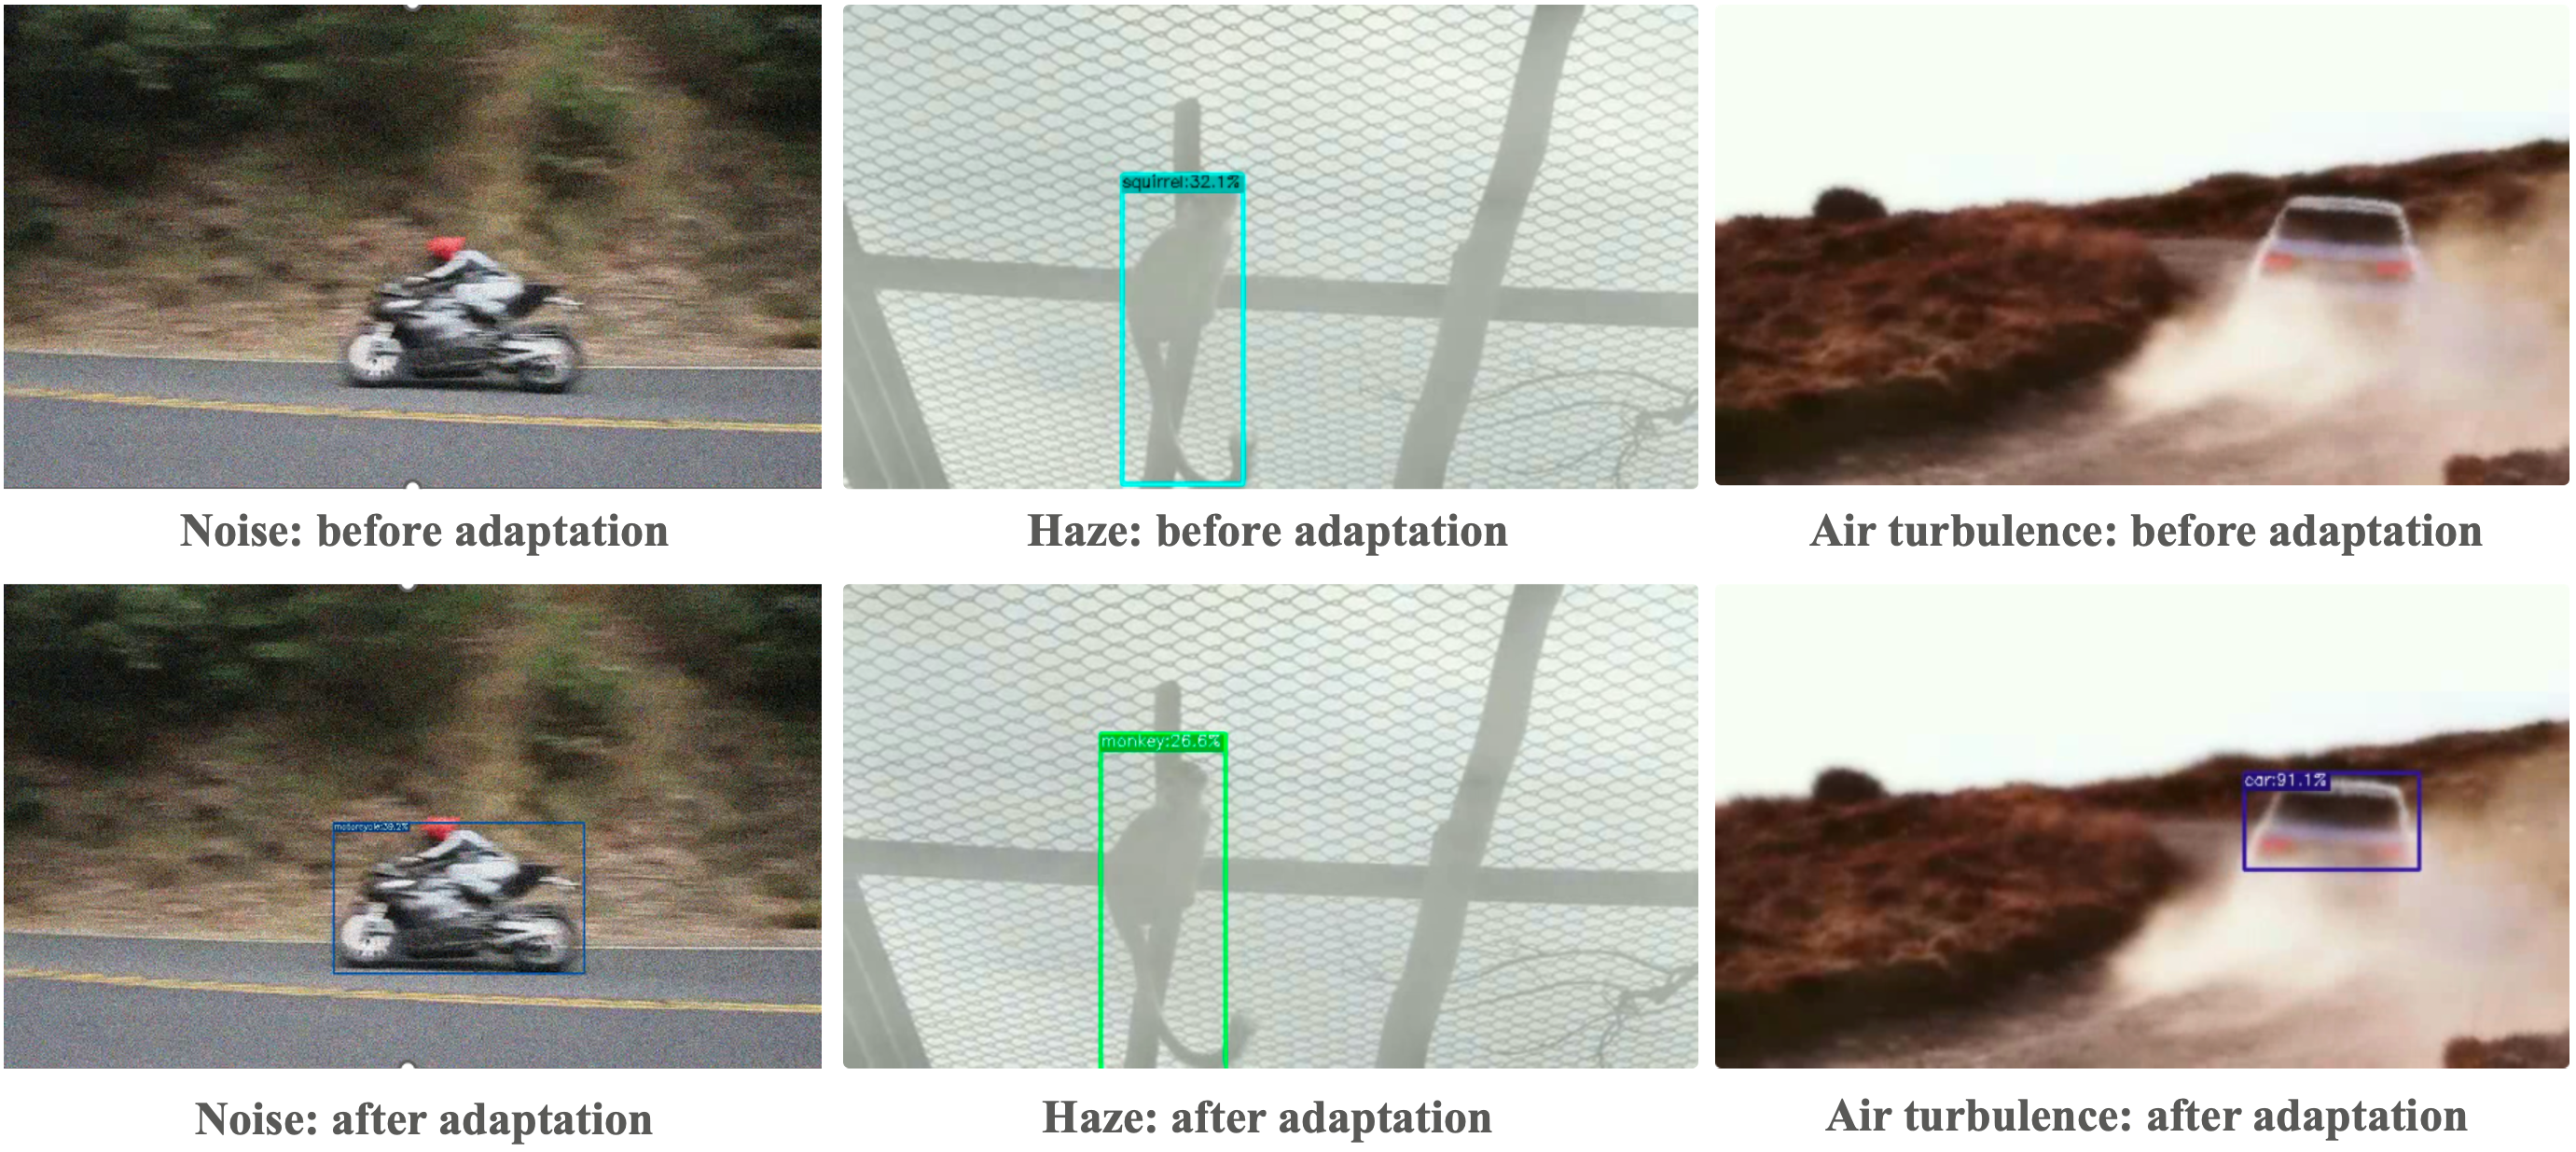
\includegraphics[width=\linewidth]{figures/effect.png}%
\caption{Visual comparison before and after the SFDA by STAR-MT. All experiments are conducted with YOLOV-S.}
\label{fig:effect}
\end{figure*}

Following its publicly available codebase, we trained the YOLOV in all three scales — small (S), large (L), and extra-large (X) — using the source dataset. In our experiment, the post-processing method was omitted as it does not pertain to our algorithms. These models were then directly tested on target domains, with the findings detailed in Table \ref{table:overall}. The Average Precision at $50\%$ threshold (AP50) on the source domain is registered as $77.3\%$, $83.6\%$, and $85.0\%$ for YOLOV-S, YOLOV-L, and YOLOV-X, respectively. The significant degradation in performance, when we test the source-train model on the target domain dataset, indicates that challenging image conditions markedly reduce the performance of the VOD models.

In addition to the initial training, we used a supervised approach to fine-tune the source-trained YOLOV models on the target domain datasets. This supervised fine-tuning serves as a theoretical benchmark for the upper limit of performance achievable through unsupervised adaptation. Deviating from the original pipeline, which involves training the base detector prior to the temporal aggregation module, we discovered that directly fine-tuning the temporal aggregation module leads to improved outcomes. Therefore, our fine-tuning focuses solely on the temporal aggregation module for the target domains, as detailed in \cite{shi2023yolov}. The results of this supervised fine-tuning, labeled as ``oracle", are also presented in Table \ref{table:overall}.

Before implementing the mean-teacher-based methods, we conducted a preliminary experiment with the pseudo-label (PL) algorithm. In this approach, models trained on the source domain are employed to process all videos in the target domain's training set, generating initial predictions. They are then filtered by threshold 0.5 on the product of objectiveness and the maximal class scores to generate pseudo labels. Since fine-tuning the single-frame backbone always causes catastrophic failure, we fixed the parameters in the backbone module and only trained the temporal aggregation module with pseudo labels. After training, we utilized the self-entropy \cite{li2021free} as the indicator to select the potential best model. The result is also demonstrated in Table \ref{table:overall}.

\subsection{Implementation details of STAR-MT}
Adhering closely to the YOLOV codebase, we maintained most of the original settings unaltered. For hyperparameter configuration, we empirically set the teacher model's smoothing coefficient, $\alpha$, to 0.9995 and the weighting factor, $\gamma$, of the $\mathcal{L}_{cls}$ to 0.2. The model training was executed using Stochastic Gradient Descent (SGD) with a batch size of 1 over 10,000 iterations. We initialized the learning rate at $2 \times 10^{-4}$ and applied a cosine annealing scheduler, tapering it down to $1 \times 10^{-4}$. In the evaluation phase, only the teacher model was utilized for inference. The mean Average Precision (mAP) was calculated with an IoU threshold of 0.5. All experiments are conducted on NVIDIA 3080 Ti and V100 GPUs.

\begin{figure}[t]
\small
\begin{minipage}[b]{.49\linewidth}
  \centering
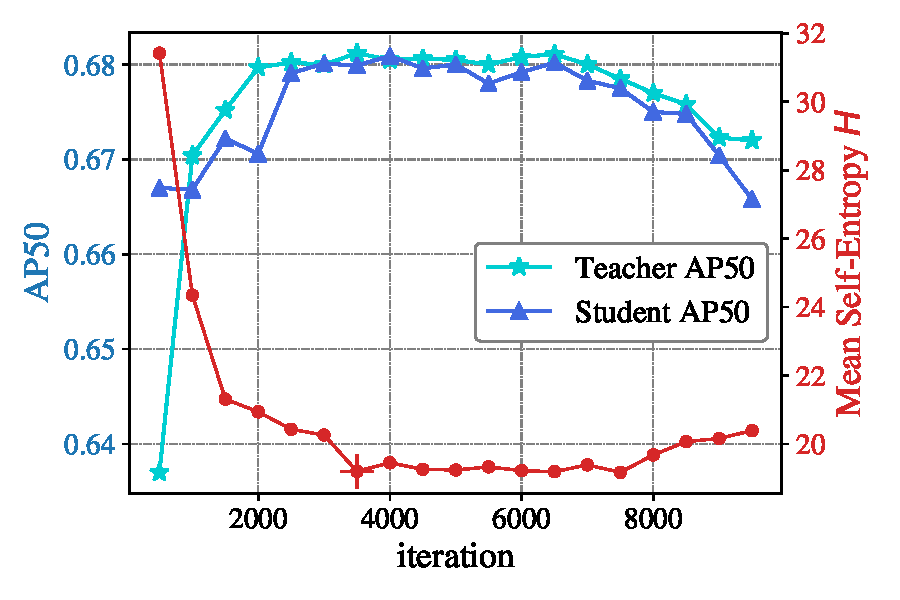
\includegraphics[width=\linewidth]{figures/yolovs.pdf}%
  \vspace{0.1cm}
  \centerline{(a) YOLOV-S}
\end{minipage}
\hfill
\begin{minipage}[b]{0.49\linewidth}
  \centering
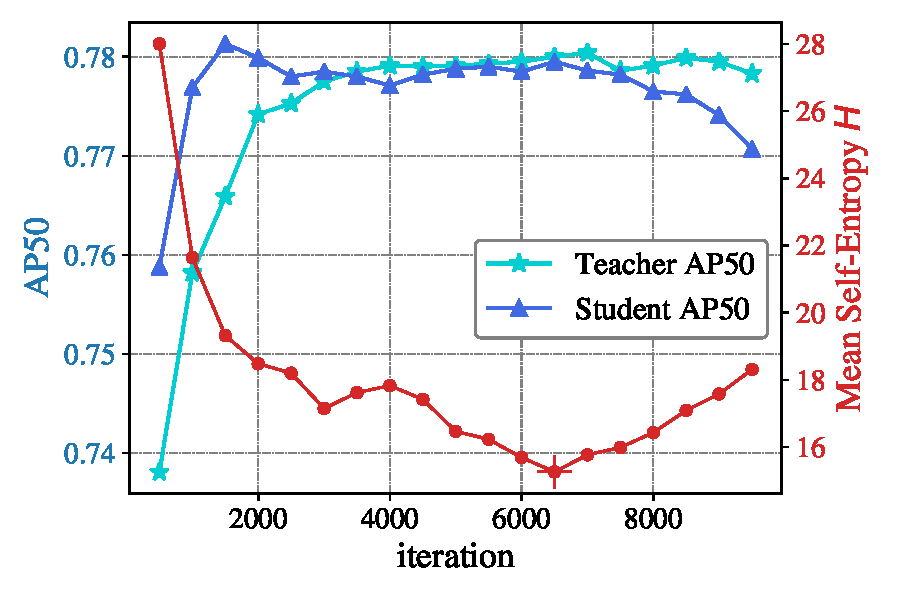
\includegraphics[width=\linewidth]{figures/yolovl.pdf}%
  \vspace{0.1cm}
  \centerline{(b) YOLOV-L}
\end{minipage}
\caption{The teacher model's AP50 and mean self-entropy $H$ variation in the STAR-MT training of YOLOV-S and YOLOV-L. Both experiments are conducted on clean $\rightarrow$ haze. The $H$ indicating the best teacher model are marked in the figures with ``\textcolor{red}{+}".}
\label{fig:curve}
\end{figure}

For each sequence in our domain adaptation experiments, 32 frames are loaded. Mosaic augmentation was disabled for all these experiments. However, we have retained both random flip and perspective transformations, applying these consistently to both weakly and strongly augmented sequence pairs. The key distinction between weak and strong augmentation lies in the strength of random chromatic transformation. Random erasing is involved only in the strong augmentation. In the TRS, random masking is applied to restrict the temporal information the student model can access, compelling it to enhance the temporal aggregation capability. The masking rate is $r\%$ where $r$ is randomly sampled from $[0, 75]$.

The performance of the STAR-MT method is demonstrated in Table \ref{table:overall}. Our method shows a significant improvement in the SFDA for VOD under all three adverse image conditions. It also demonstrates a clear advantage over conventional methods like pseudo-labeling and basic mean-teacher learning. Notably, although the method seems straightforward and not complicated, \textit{the performance of our method closely approaches that of supervised fine-tuning}. To illustrate the correlation between mean self-entropy $H$ and the performance of SFDA, we drew the variations in model performance alongside the change in $H$ value on the evaluation set, as shown in Fig \ref{fig:curve}. The $H$ values were calculated using a sliding window average over 100 iterations. We can observe the lowest value of $H$ aligns well with the peak performance of the model.


\subsection{Ablation study}
\noindent \textbf{Efficacy of alternate refinement.} One major novelty in this paper is the spatial refinement stage, as an alternately updated module in addition to the normal mean teacher learning framework. The key insights behind this are 1) temporally enhanced features of the teacher model can be used to generate reliable pseudo labels for the training of the single-frame detection head, and 2) training the single-frame detection head under the YOLOV setting is suboptimal. Thus, it needs additional guidance. From the comparison between the basic mean-teacher method (TRS only) and the proposed STAR-MT in Table \ref{table:overall}, we can verify the efficacy of alternate refinement with the spatial refinement stage. To demonstrate that the pseudo labels from the YOLOV are of higher quality, we conducted source-free domain adaptation for the YOLOX. We follow the mean-teacher framework and use the pseudo labels generated by YOLOX and YOLOV to guide the training of the student network. The result is shown in Table \ref{tab:SRS}. The model guided by the temporally refined labels in YOLOV gets better performance, which provides evidence for the efficacy of SRS.

% \noindent \textbf{Effectiveness of weight initialization for the student model.} The teacher
% model serves as a performance lower bound for the student model \cite{liu2023periodically}. Observing that the performance of teacher model is better than the student model in most iterations, we update the weight of the student model by that of the teacher model in the beginning of each stage. We evaluate the effect in Table, which 
\begin{table}
    \centering
    \begin{tabular}{l|c|c}
    \hline
        Model & YOLOX-S &  YOLOX-L  \\
        \hline
        Source-only  & 35.9 & 56.6  \\
        PL guided by YOLOX  & 49.2 & 61.3  \\
        PL guided by YOLOV & 51.0 & 62.9\\
        \hline 
        Oracle & 56.7 & 66.0 \\
    \hline
    \end{tabular}
    \caption{The efficacy of YOLOV as the teacher model for the SFDA of the single-frame detection backbone. All experiments are conducted on clean $\rightarrow$ noise. The metric is AP50(\%), the larger, the better.}
    \label{tab:SRS}
\end{table}


\begin{table}
    \centering
    \begin{tabular}{c|c|c|c|c}
    \hline
        $\mathcal{L}_{MSE}$ & $\mathcal{L}_{BCE}$ & $\mathcal{L}_{cls}$ & YOLOV-S  & YOLOV-L \\
        \hline
        \xmark & \cmark & \cmark & 62.1 & 71.5 \\
        \cmark & \cmark & \xmark & 67.6 & 77.4 \\
        \cmark & \xmark & \cmark & 67.8 & 77.3 \\
        \cmark & \cmark & \cmark & \textbf{68.1} & \textbf{78.0} \\
    \hline
    \end{tabular}
    \caption{The efficacy of losses. All experiments are conducted on clean $\rightarrow$ haze. The metric is AP50(\%), the larger, the better.}
    \label{tab:losses}
\end{table}

\noindent \textbf{Efficacy of losses.} In our study, the three utilized loss functions are categorized as feature alignment loss $\mathcal{L}_{MSE}$ and pseudo-label based losses ($\mathcal{L}_{BCE}$ and $\mathcal{L}_{cls}$). We experimented with various reasonable combinations of these loss terms to assess their impact. In all combinations, at least one pseudo-label-based loss was maintained. The results are detailed in Table \ref{tab:losses}. Initially, we excluded the feature alignment loss $\mathcal{L}_{MSE}$ and observed a significant decline in adaptation performance. This indicates the model's high sensitivity to label quality and the importance of restricting the feature space generated by the detection head. Further, we excluded $\mathcal{L}_{MSE}$ and $\mathcal{L}_{cls}$ separately to evaluate their individual contributions. The results confirmed the effectiveness of both losses.

\begin{table}
    \centering
    \begin{tabular}{c|c|c|c|c}
    \hline
        Model & $\tau = 50$ & $\tau = 100$ & $\tau = 200$  & $\tau = 500$ \\
        \hline
        YOLOV-S & 68.0 & \textbf{68.1} & 67.6 & 67.8 \\
        YOLOV-L & 76.9 & 77.5 & \textbf{78.0} & 77.7 \\
        YOLOV-X & 78.2 & 78.4 & \textbf{78.9} & 78.8 \\
    \hline
    \end{tabular}
    \caption{The impact of the number of iterations in each stage. All experiments are conducted on clean $\rightarrow$ haze. The metric is AP50(\%), the larger, the better.}
    \label{tab:iteration}
\end{table}

\noindent \textbf{Number of iterations for each stage.} We also evaluated the optimal number of fine-tuning iterations, $\tau$, for each stage within a period. For this purpose, we conducted experiments that set $\tau$ to various values: 50, 100, 200, and 500, while maintaining 10,000 training iterations. The determination of optimal results within this range was based on the mean self-entropy $H$ values, where the teacher model associated with the first local minima of $H$ is selected. This assessment was carried out across all three model scales, and the findings are presented in Table \ref{tab:iteration}. The results indicate that different scales of the model may require distinct hyperparameters to achieve optimal adaptation performance.